\chapter{Signalverarbeitung bei ballistokardiographischen Signalen}

Im folgenden Kapitel wird eine Einführung in das Thema der Signalverarbeitung und besonders Artefakterkennung bei ballistokardiographischen Signalen gegeben. Hierzu wird zunächst Grundlegendes zu der Verarbeitung kardiorespiratorischer Signale erläutert. Ein in dieser Arbeit verwendeter Algorithmus zur Detektion von Herzschlägen wird vorgestellt. Anschließend wird die Thematik der Artefakterkennung eingeführt und der aktuelle Stand der Wissenschaft bei \ac{BKG}-Signalen vorgestellt. Hierfür werden drei Verfahren im Detail betrachtet. Darüber hinaus werden die in dieser Arbeit untersuchten Daten vorgestellt und die durchgeführte Vorverarbeitung beschrieben.

\section{Grundsätzliches} % TODO: eventuell in allgemeinen Teil des Kapitels

	Kardiorespiratorische Signale sind durch die quasiperiodische Natur des Herzens selbst quasiperiodisch. Zwei zyklische Vorgänge werden gleichzeitig gemessen, lassen sich aber durch eine Bandpass-Filterung nach ihren unterschiedlichen Frequenzen filtern. Der Normbereich für die Atemfrequenz liegt bei 12 bis 25 Atemzügen pro Minute, alles ober- und unterhalb wird als abnormal betrachtet. Bei der Herzfrequenz wird ein Bereich von 30 bis 200 Schlägen pro Minute erwartet. Dabei entsprechen 30 Schläge pro Minute der Pulsabsenkung in der Nacht, der Ruhepuls selbst ist höher. Grundsätzlich gibt es verschiedene Arten der Signalverarbeitung: Algorithmen, die im Zeitbereich arbeiten, solche, die im Frequenzbereich arbeiten und solche, die beides kombinieren. Dabei ist zu beachten, dass bei frequenzbasierten Algorithmen durch die Analyse von spektralen Eigenschaften zunächst nur durchschnittliche Frequenzen ermittelt werden. Dies ist für einige medizinische Anwendungen ausreichend, für andere wie z.B. die Ermittlung der \ac{HRV} allerdings nicht. Algorithmen, die auf dem Zeitbereich arbeiten basieren oft auf Wissen über die Morphologie des physiologischen Signals. Durch die Eigenschaften der \ac{BKG}-Signale, vor allem durch die variable Morphologie ist dies schwieriger als bei anderen kardiorespiratorischen Signalen. \citeauthor{Paalasmaa2015} sagt dazu:

	\begin{quote}\textit{The properties of the BCG signal vary so much in practice that no simple filtering rule can be devised for an accurate and reliable beat-to-beat interval detection}\footcite{Paalasmaa2015}\end{quote}
	
	Diese Aussage gilt sowohl für die Detektion von Schlag-zu-Schlag Intervallen als auch für die Beurteilung der Signalqualität, bzw. die Artefakterkennung.

\section{Detektion von Herzschlägen}\label{CLIE}

	In dieser Arbeit wird der von \citeauthor{Bruser2013} entwickelte Algorithmus, der \textit{Continuous Local Interval Estimator}, kurz \textit{CLIE} verwendet. Aus diesem Grund wird er hier vorgestellt. Der Algorithmus beruht auf der in \ref{ballistokardiographie} erwähnten Annahme, dass sich aufeinander folgenden Herzschläge ähneln und schätzt die Herzrate anhand der Selbstähnlichkeit des Signals.


	Der Algorithmus iteriert mit einem \textit{Moving window} über das mit einem Bandpass gefilterte Signal. Es werden zwei Schwellwerte für die Intervalllänge $T$ genutzt, $T_{min}$ und $T_{max}$, basierend auf dem bekanntem Bereich der Herzrate von 30 bis 200 Schlägen pro Minute. Die Länge des Analysefensters $w_i$ entspricht $2 * T_{max}$, sodass mindestens zwei vollständige Herzschläge enthalten sind.
	\[w_i[v] = x[n_i + v], v \in \{ -T_{max} * f_s, ..., T_{max} * f_s\}\]
	
	In jedem Fenster wird die lokale Intervalllänge $T_i$ geschätzt und anschließend das Zentrum des Fensters $n_i$ weiterbewegt: \[ n_{i+1} = n_i + \Delta t * f_s \].
	
	Die Schätzung der Intervalllänge beruht auf drei Selbstähnlichkeitsmaßen, die wie folgt definiert sind:
	
	\begin{align*}
		E\textsubscript{Corr}[N] &= \frac{1}{N} \sum_{v=0}^{N} w[v]w[v-N],\\
		E\textsubscript{AMDF}[N] &= (\frac{1}{N} \sum_{v=0}^{N} |w[v]-w[v-N]|)^{-1},\\
		E\textsubscript{MAP}[N] &= \max_{v \in \{0,...,n\}}(w[v]+w[v-N]).
	\end{align*}
 	
 	Dabei berechnet $E_{corr}$ eine modifizierte Autokorrelationsfunktion, mit $E_{AMDF}$ wird die Differenz des Signals zueinander miteinbezogen und mit $E_{MAP}$ werden die maximale Amplituden von beliebigen 2 Samples über das ganze Fenster berechnet. AMDF steht für \textit{modified average magnitude difference function} und MAP für \textit{maximum amplitude pairs}. Diese Schätzer entsprechen jeweils einer Wahrscheinlichkeitsfunktion, die beschreibt wie wahrscheinlich es ist, dass $n$ dem tatsächlichen Schlag-zu-Schlag-Intervall entspricht. Durch Skalierung können sie in Wahrscheinlichkeitsdichtefunktionen verwandelt werden. Durch Kombination dieser drei Funktionen wird nun der wahrscheinlichste Wert für $N$ ermittelt:
 	\[ N_{opt} = \argmax_{N} p(N|E\textsubscript{Corr}, E\textsubscript{AMDF}, E\textsubscript{MAP}) \]
 	
	Nach dem Satz von Bayes kann die Wahrscheinlichkeit, dass $N$ der tatsächlichen Intervalllänge entspricht, auch wie folgt ausgedrückt werden:
	
	\[
		p(N|E\textsubscript{Corr}, E\textsubscript{AMDF}, E\textsubscript{MAP}) = \frac{p(E\textsubscript{Corr}, E\textsubscript{AMDF}, E\textsubscript{MAP} | N) p(N)}{p(E\textsubscript{Corr}, E\textsubscript{AMDF}, E\textsubscript{MAP})}
	\]
	
	Da $p(E\textsubscript{Corr}, E\textsubscript{AMDF}, E\textsubscript{MAP})$ unabhängig von $N$, kann es für die Ermittlung der wahrscheinlichsten Intervalllänge $T_{opt}$ vernachlässigt werden. Unter den Annahmen, dass die Ergebnisse der drei Schätzer nicht voneinander, sondern nur von $N$ abhängen und dass $N$ gleichverteilt ist, kann $T_opt$ wie folgt ermittelt werden:
	
	\begin{align*}
		E_f[N] &= E\textsubscript{Corr}[N] \cdot E\textsubscript{AMDF}[N] \cdot E\textsubscript{MAP}[N],\\
		N_{opt} &= \argmax_{n} E_f[N]	
	\end{align*}
	
	Durch lineare Skalierung erhält man auch hier eine Dichtefunktion. Abbildung \ref{fig:estimator-fusion} zeigt die 3 einzelnen Dichtefunktionen und die fusionierte Fusion. In letzterer zeigt ein deutlicher Hochpunkt $N_{opt}$.
	
	 \begin{figure}[H]
		\centering
		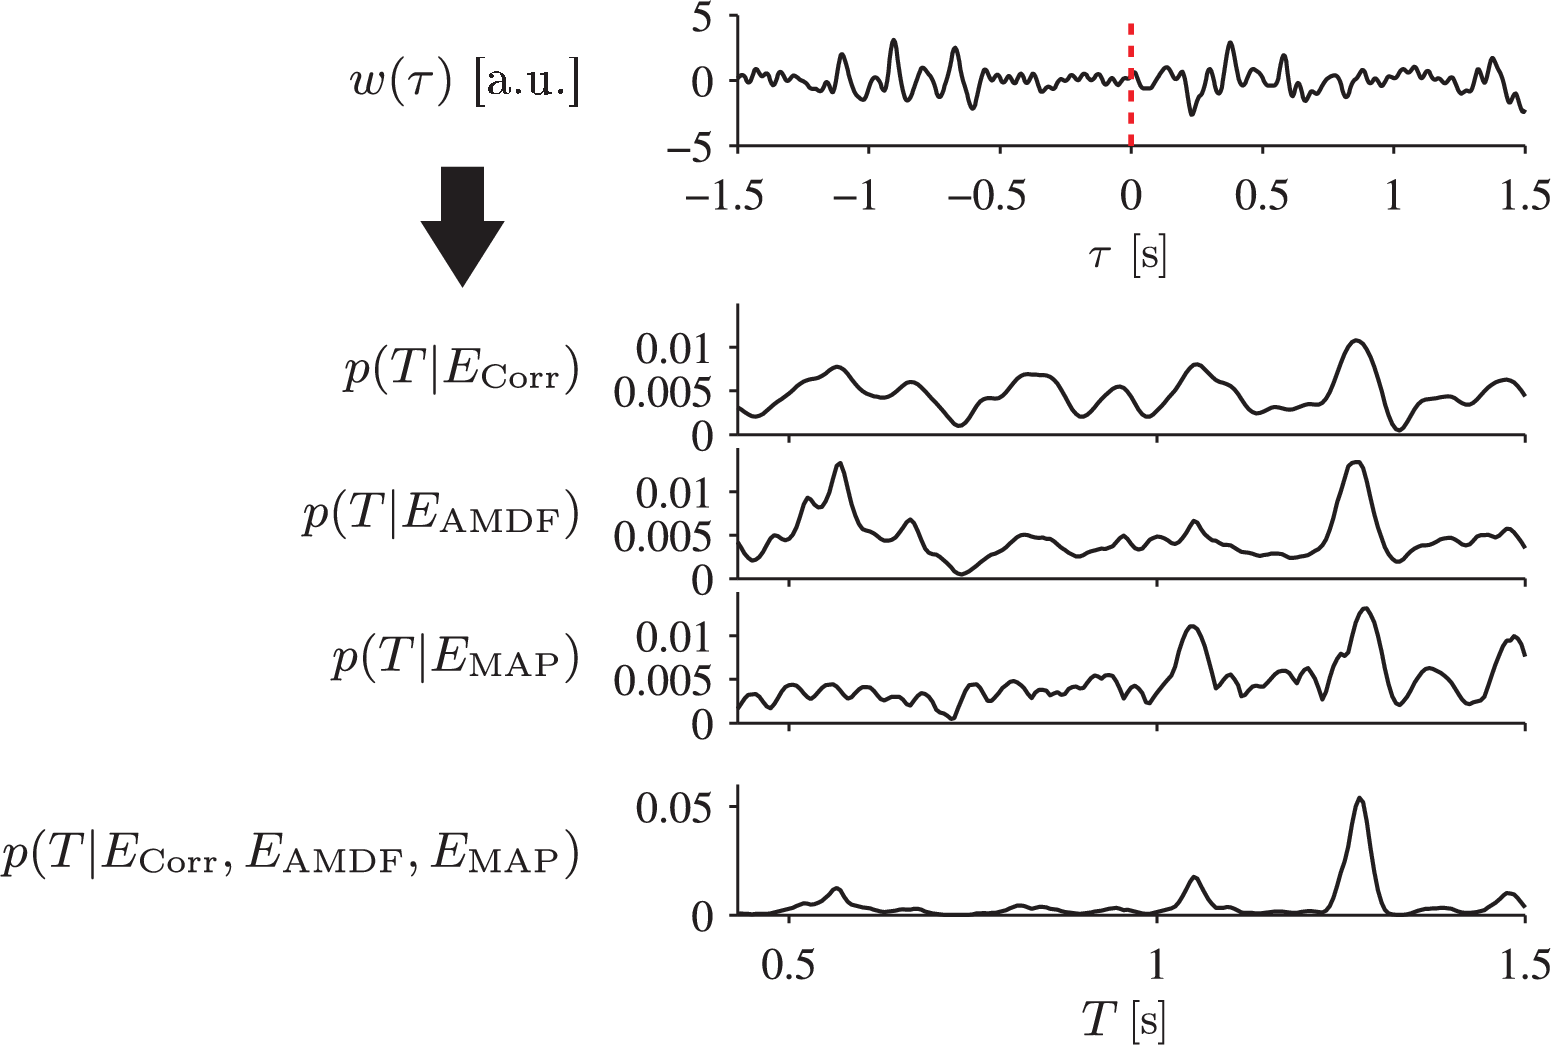
\includegraphics[width=0.5\textwidth]{pic/estimator-fusion.png}
		\caption[Intervallschätzer nach \citeauthor{Bruser2013}]{Die drei Intervallschätzer und ihre Fusion}
		\label{fig:estimator-fusion}
	\end{figure}
	
	Nun gibt es für jeden Punkt im Signal eine Schätzung der Intervalllänge. Mit Hilfe der Fenstergröße und dieser Länge können die zu einem Herzschlag gehörenden Hochpunkte ermittelt werden, nämlich die, die die größte kombinierten Amplitude mit dem durch die Intervalllänge gegebenen Abstand besitzen. Für jeden dieser Punkte $P_k$ existiert nun eine Menge an Schätzungen $T_k$, mit der eine robuste Intervallschätzung $\overline{T_k} = \text{median}(T_k)$ ermittelt werden kann.\footcites[Vgl. zu diesem Kapitel][]{Bruser2013}

\section{Artefakterkennung}
	
	Artefakte bzw. Signal von geringer Qualität sind irrelevante Signalteile mit variierender Amplitude, Frequenz und Dauer, die das physiologische Signal stören\footcite[Vgl.][]{Nizami2013}. Das Ziel der Artefakterkennung ist es, nur die Teile des Signals zu verarbeiten, die Vitalparameter enthalten. Bewegungsartefakte, Sensorstörungen und ähnliches, die diese Parameter überlagern, sollen die Verarbeitung nicht beeinflussen. Dabei ist die Quelle der Störung selbst irrelevant, allerdings sollten keine medizinisch induzierten Abnormalitäten als gestörtes Signal klassifiziert werden. \citeauthor{Sadek2016} unterscheidet zwischen informativem und nicht-informativem Signal. Informatives Signal enthält \textit{noise} und Signal von guter Qualität und Vitalparameter können ohne weiteres extrahiert werden. Im Gegensatz dazu sind die Informationen bei nicht-informativem Signal so mit Artefakten und \textit{noise} vermischt, dass vor Extraktion der Vitalparameter weitere individuelle Verarbeitung nötig ist oder die Extraktion von physiologischen Eigenschaften gar unmöglich ist. Teils wird die Signalqualität auch mit so genannten \acp{SQI} gemessen, die je nach \ac{SQI} und Anwendungsfall verschiedene Aussagen haben. Im klinischen Kontext genutzte Artefakterkennung verwendet oft relativ einfaches Preprocessing.\footcite[Vgl.][]{Nizami2013} Außerdem sind in den meisten Algorithmen bestimmte Informationen direkt oder indirekt \textit{hard coded}. Das kann zum einen etwas wie Typ oder Frequenz der Daten sein, aber auch demographische Informationen über die Patient*innen wie Alter, Gewicht oder medizinischer Zustand.\footcite[Vgl.][]{Nizami2013}
		
	\begin{figure}[H]
		\centering
		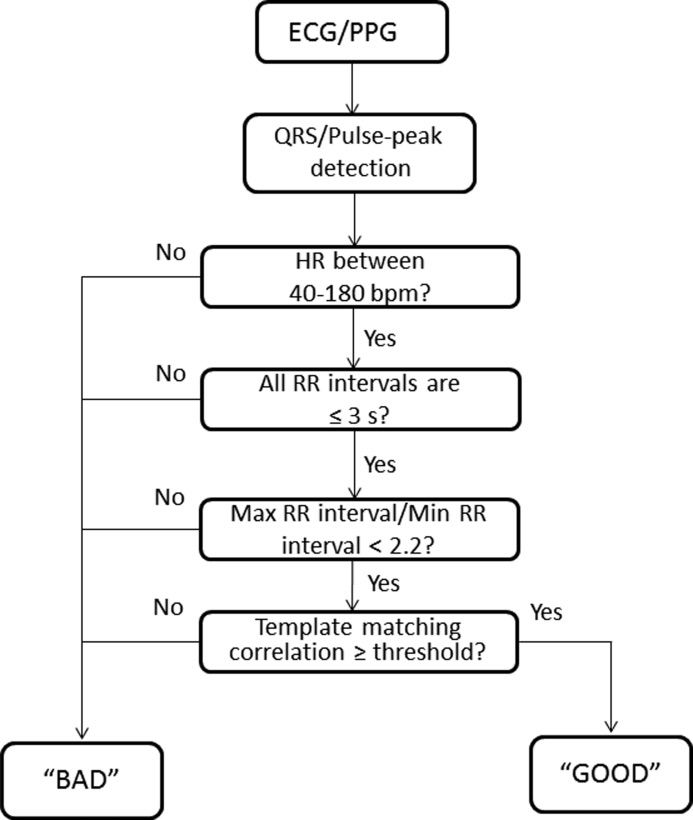
\includegraphics[width=0.5\textwidth]{pic/ad_flussdiagramm}
		\caption[Flussdiagramm eines Algorithmus zur Beurteilung der Signalqualität]{Flussdiagramm eines Algorithmus zur Beurteilung der Signalqualität\protect\footnotemark}
		\label{fig:ecg-ad}
		\footnotetext{Entnommen aus \cite{Orphanidou2015}.}
	\end{figure}
	
	Um einen Eindruck über übliche Beurteilung der Signalqualität bei anderen kardiorespiratorischen Signalen zu bekommen, wird in Abbildung \ref{fig:ecg-ad} ein Beispiel für \ac{EKG} und \ac{PPG} gezeigt. In jeweils 10-Sekunden Fenstern wird zunächst eine Segmentierung der Herzschläge durchgeführt und anschließend vier Kriterien überprüft, die jeweils ausreichend sind, um die Signalqualität als schlecht zu klassifizieren. Im ersten Kriterium wird geprüft ob die Herzrate zwischen 40 und 180 Schlägen pro Minute liegt. Im zweiten Schritt wird sichergestellt, dass kein Schlag fehlt, indem geprüft wird, ob alle Intervalle kürzer als drei Sekunden sind. Eine Intervalllänge von 3 Sekunden entspräche über eine Minute einer Herzrate von 20 Schlägen pro Minute. Anschließend wird geprüft, ob die Herzrate nur in einem begrenzten Bereich variiert; das maximale Verhältnis der maximalen zur minimalen Intervalllänge muss kleiner als $2.2$ sein. Abschließend wird geprüft, ob die Korrelation mit einem erstellten Template einen gewissen Schwellwert nicht unterschreitet. Dieser Algorithmus enthält übliche Techniken der Signalbeurteilung: Eine Begrenzung der akzeptierten Herzrate und Herzratenvariabilität und dem Vergleich mit einem zuvor erstellten Template.
	
	Bei ballistokardiographischen Signalen gestaltet sich auch die Beurteilung der Signalqualität schwieriger als bei anderen kardiorespiratorischen Signalen. Zusätzlich zu der gegebenen Variabilität durch die Atmung ist eine Problematik, dass plötzliche Veränderungen der Signalmorphologie bei Positionsänderungen zuvor erstellte Templates obsolet machen und auch andere Schwellwerte nicht mehr angemessen sind. Bei Artefakten in \ac{BKG}-Signalen kann zwischen Artefakten mit hoher und mit niedriger Energie unterschieden werden. Artefakte mit hoher Energie, wie in Abbildung \ref{fig:high-energy-artifact} gezeigt entstehen, weil Bewegungen stärkere Krafteinwirkungen verursachen als Atmung und Herzschlag. Diese Tatsache wird häufig zur Erkennung dieser verwendet. Artefakte mit niedriger Energie, wie in Abbildung \ref{fig:low-energy-artifact} gezeigt, sind weniger auffällig.
	
	\begin{figure}[H]
		\centering
		\begin{minipage}{0.4\linewidth}
			\centering
      		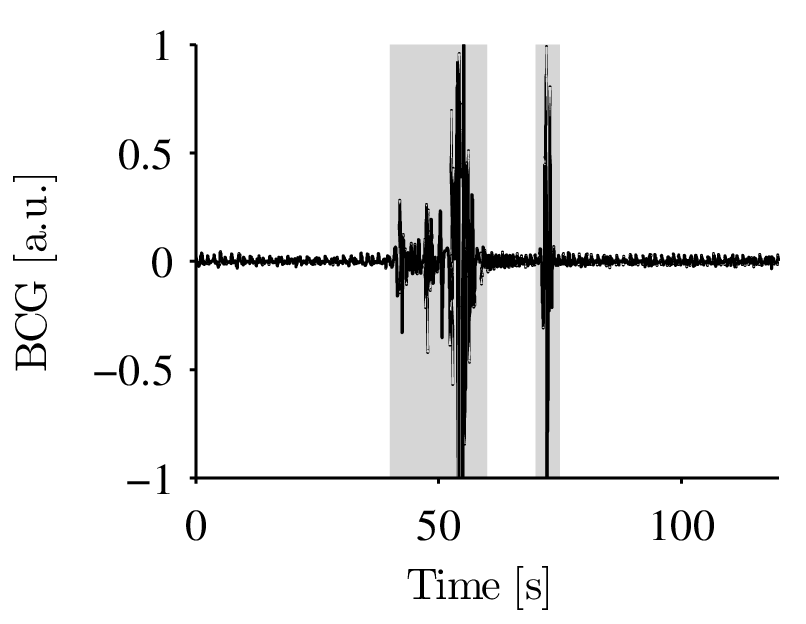
\includegraphics[width=0.9\textwidth]{pic/high-energy-artifacts.png}
			\caption[Artefakte mit hoher Energie]{Artefakte mit hoher Energie}
			\label{fig:high-energy-artifact}
    	\end{minipage}
    	\hfill
    	\begin{minipage}{0.4\linewidth}
    		\centering
      		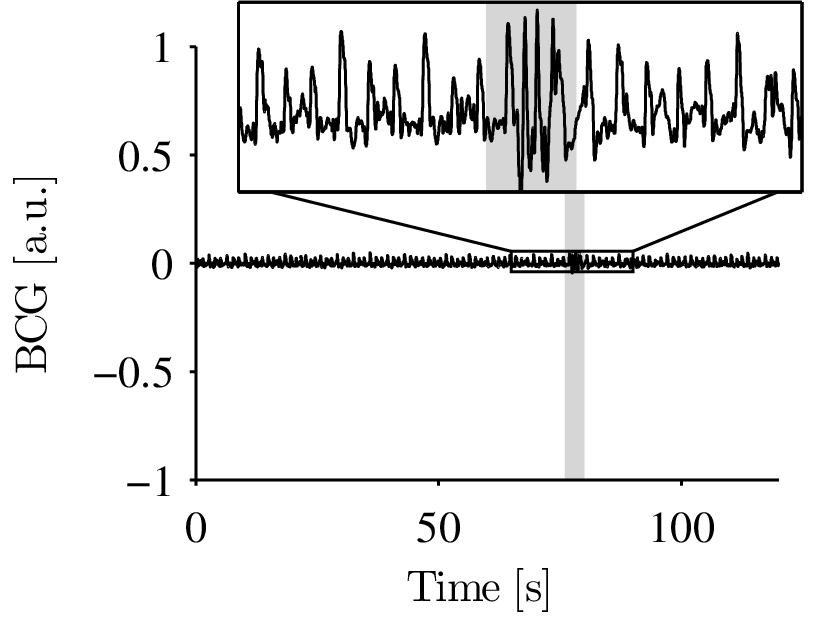
\includegraphics[width=0.9\textwidth]{pic/low-energy-artifacts.png}
			\caption[Artefakte mit niedriger Energie]{Artefakte mit niedriger Energie}
			\label{fig:low-energy-artifact}
    	\end{minipage}
	\end{figure}
	
	Bei der Betrachtung verschiedener Ansätze zur Signalverarbeitung und Artefakterkennung bei \ac{BKG}-Signalen ist auffällig, dass Proband*innen oft angewiesen, sich möglichst wenig zu beobachten. Das ist bei der Messung im Alltag, insbesondere bei Messungen in Betten nicht realistisch. Dazu kommt, dass beim Einsatz im Alltag auch Kontakt mit der Person nicht immer gewährleistet ist, z.B. wenn diese sich aufrichtet. \citeauthor{HoogAntink2020} haben festgestellt, dass bei Messsystemen in Betten besonders Messungen tagsüber große Signalteile von schlechter Qualität aufweisen, deutlich mehr als nachts. Dies ist durch gesteigerte Aktivität tagsüber erklärbar. Ebenfalls im \textit{unobtrusive} Kontext nicht zielführende Methoden zur Artefakterkennung verwenden eine \ac{EKG}-Referenz.
	
	Im Folgenden werden drei ausgewählte Methoden zur Beurteilung der Signalqualität vorgestellt.

	\subsection{Schwellwertbasierte Artefakterkennung}
	
	In \citetitle{Pino2015} präsentieren \citeauthor{Pino2015} einen Ansatz für die Erkennung von Körperbewegungen für ein in einen Stuhl eingebettetes \ac{BKG}-Messsystem. Dafür werden über ein \textit{moving window} Maximum, Minimum, Standardabweichung und Mittelwert ermittelt und daraus 2 Schwellwerte berechnet:
	
	\begin{eqnarray*}
		&T_1 &= \frac{\text{max} + \text{min}}{2},\notag\\
		&T_2 &= \text{mean} + 1,1 * \text{std}.\notag
	\end{eqnarray*}
	
	Die Länge des \textit{moving window} ist mit 200 Samples bei einer Abtastrate von 200 Hz benannt. Untersucht wurden sowohl Freiwillige im Labor, als auch im Krankenhauswartezimmer für eine sehr kurze Messdauer von ein bis zwei Minuten. Mit diesem Ansatz wurde bei mehr als 50 \% der Laborgruppe eine \textit{Coverage} zwischen 87 \% und 95 \% erreicht. Die \textit{Coverage} der im Krankenhaus aufgenommenen Gruppe war bedeutend niedriger; hier lagen 50 \% der Messungen zwischen 48 \% und 95 \% \textit{Coverage} erreicht. Zu der Genauigkeit der Herzschlagdetektion auf den akzeptierten Signalteilen wird keine Aussage in Zahlen getroffen, sondern nur der folgende Bland-Altman Graph gezeigt.
	
	\begin{figure}[H]
		\centering
		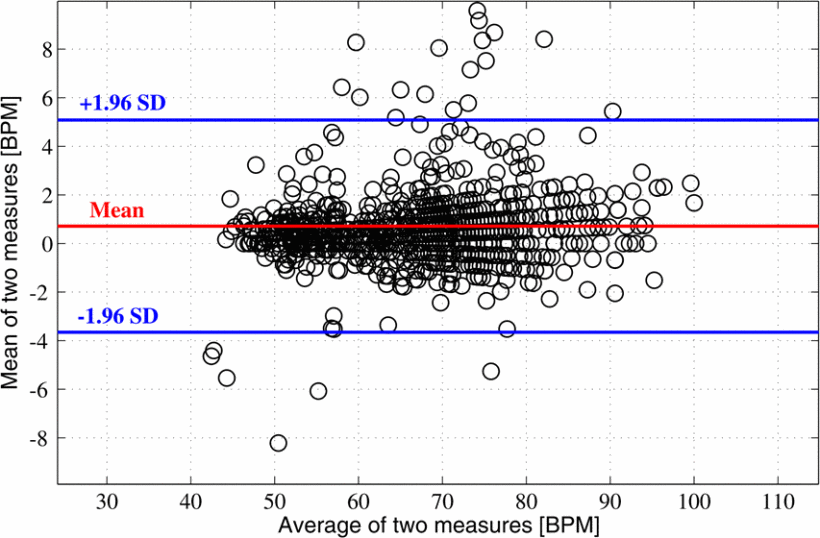
\includegraphics[width=0.5\textwidth]{pic/bland-altman-pino.png}
		\caption[Genauigkeit der Herzratenberechnung bei schwellwertbasierter Artefakterkennung]{Bland-Altman Graph zwischen von \ac{EKG} und \ac{BKG} berechneter \ac{HR}}
		\label{fig:bland-altman-pino}
	\end{figure}
	
	Hier zeigt sich, dass beim Großteil des hier betrachteten Signals die \ac{HR} größtenteils mit einer Genauigkeit von $\pm 3$ Schläge pro Minute bestimmt werden konnte. Allerdings handelt es sich hier um im Sitzen aufgenommenes Signal, bei dem die Variabilität geringer ist als bei in Betten aufgenommenem \ac{BKG}.
	
	
	\subsection{Maschinelles Lernen mit statistischen Merkmalen}
	
	Ein Algorithmus zur Beurteilung der Signalqualität mittels maschinellen Lernens wird von \citeauthor{Sadek2016} im Paper \citetitle{Sadek2016} beschrieben. Betrachtet werden \ac{BKG}-Signale, die in einem Massagesessel aufgenommen werden, also ebenfalls im Sitzen aufgenommenes Signal, bei dem eine geringere Variabilität als in unserem Anwendungsfall erwartet wird.
	
	Die vorliegenden Daten wurden manuell von Expert*innen als informativ oder nicht informativ klassifiziert und in 10-Sekunden-Segmente, die sich nicht überlappen, aufgeteilt, die sich nicht überlappen. Insgesamt waren 58 \% der Daten als informativ und 42 \% als nicht-informativ gelabelt. Von diesen Segmenten wurden nach einer Bandpass-Filterung auf 1 bis 12 Hz 13 statistische Merkmale berechnet:
	%\begin{multicols}{2}
	\begin{itemize}
		\item Minimun
		\item Maximum
		\item Mittelwert
		\item Standardabweichung
		\item Schiefe
		\item Kurtosis
		\item Spannweite
		\item Interquartilspannweite
		\item mittlere absolute Abweichung
		\item Anzahl der Nulldurchgänge
		\item Varianz der lokalen Minima
		\item Varianz der lokalen Maxima
		\item Mittelwerte der Signalhüllkurve\footnote{Die Signalhüllkurve ist eine glatte Kurve, die die Extrema des Signals umreißt.}
	\end{itemize}
	%\end{multicols}
	
	Für fünf verschiedene Modelle des maschinellen Lernens wurden jeweils die besten Hyperparameter über Kreuzvalidierung auf den Trainingsdaten ermittelt und die Modelle anschließend mit diesen Hyperparametern trainiert. Anschließend wurden die Modelle auf unbekannten Daten getestet. Das Training und Testen wurde mit getauschten Gruppen wiederholt. Das beste Ergebnis wurde mit einem Random Forest erreicht: Die durchschnittliche Genauigkeit der Kreuzvalidierung betrug $98,13 \% $ bzw. $100 \%$ bei getauschten Gruppen. Auf dem Testset wurde eine Genauigkeit von $92,3 \%$ bzw. $97,99 \%$ erreicht. Weitere Evaluationsmetriken außer eine \textit{Confusion Matrix} für den besten Klassifikator sind nicht gegeben.
	
	Diese Ergebnisse sind sehr gut, allerdings muss bei der Einordnung beachtet werden, dass bei für die Kreuzvalidierung die Segmente zufällig verteilt wurden und nicht beachtet wurde, dass der Algorithmus für aussagekräftige Validierung einzelne Personen nicht darf. Dadurch ist die Performance auf gänzlich unbekannten Daten weiterhin nicht bekannt und vermutlich schlechter, als die Zahlen es hier vermuten lassen.
	
	\subsection{Ähnlichkeit der Intervallschätzer des CLIE-Algorithmus}\label{brueserQI}
	
	Ein weiteres Maß für die Signalqualität basiert auf dem in \ref{CLIE} vorgestellten Algorithmus zur Intervallschätzung. Dieser \acl{SQI} misst, wie einig sich die drei Intervallschätzer sind. Wenn diese sich uneinig sind, ist der \ac{SQI} bei 0, je ähnlicher sich die Schätzungen sind, desto höher ist er. Für jedes Fenster $i$ wird er wie folgt berechnet: \[ q = \frac{E_f[n_{opt}, i]}{\sum E_f[n, i]} \]
	
	Bei der Ermittlung der konkreten Schlag-zu-Schlag Intervalle wird von $q$ äquivalent zu den geschätzten Intervalllängen der Median berechnet. Schätzungen dessen Qualität unter einem Schwellwert $q_{th}$ werden verworfen. Die Wahl von $q_{th}$ hängt von der gewünschten Genauigkeit und \textit{Coverage} ab, je höher die gewünschte Genauigkeit, desto niedriger die \textit{Coverage}.
	
	Dieser \ac{SQI} wird in verschiedenen Papern mit unterschiedlich gewähltem $q_{th}$ genutzt und erreicht damit bei der \ac{BKG}-Messung in Betten während der Nacht bei gesunden Patient*innen gute Ergebnisse. \citeauthor{Bruser2013} erreicht zum Beispiel bei 8 gesunden Proband*innen durchschnittlich eine \textit{Coverage} von $85 \%$ bei einem Fehler zur \ac{EKG}-Referenz von $0.61 \%$.\footcite[Vgl.][]{Bruser2013} Bei Patient*innen im Krankenhaus zeigte sich, dass sowohl die Ergebnisse bezüglich der \textit{Coverage} als auch der Genauigkeit bedeutend schlechter sind. So erreichte \citeauthor{HoogAntink2020} bei 14 Patient*innen durchschnittlich $40 \%$ \textit{Coverage} bei einem Fehler von $2.16 \%$. Werden nur die nächtlichen Aufnahmen betrachtet, wird eine \textit{Coverage} von $52 \%$ bei einem Fehler von $1.29 \%$ erreicht. Bei der Berechnung letztere Ergebnisse wurden zusätzlich Intervallschätzungen verworfen, deren relative Abweichung vom Median der anderen Schätzungen einen bestimmten Schwellwert überschreitet.\footcite[Vgl.][]{HoogAntink2020}
	
	Dieser Algorithmus ist der einzige der drei betrachteten, der im Bett aufgenommenes \ac{BKG}-Signal untersucht. Die Ergebnisse sind bei gesunden, schlafenden Patient*innen sehr gut, im tatsächlichen Einsatz im Krankenhaus wird allerdings eine deutlich geringere \textit{Coverage} bei höherem Fehler erreicht.
	
\section{Messdaten}

	Die vorliegenden Messdaten wurden in der Gefäßstation des Universitätskrankenhauses in Tampere (Finnland) aufgenommen und wurden im Paper \citetitle{HoogAntink2020} bereits untersucht. Insgesamt wurden 14 Patient*innen, zwei weiblich und zwölf männlich, bis zu 24 h überwacht. Alle hatten sich verschiedenen gefäßchirurgischen Eingriffen unterzogen. Das Durchschnittsalter der Patient*innen betrug $69.57$ Jahre und die durchschnittliche Messdauer $17.7$ h, wobei sie zwischen $4.46$ und $22.96$ h variierte.
	
	Gemessen wurde mit einem EMFit QS Bettsensor, der zwischen der Matratze des Krankenhausbettes und dem Bettgestell positioniert wurde. Die Abtastrate des \ac{BKG} betrug 100 Hz. Das Referenz-\ac{EKG} wurde mit einem Faros 360 Patientenmonitor mit einer Abtastrate von 1 kHz aufgenommen und hat drei Kanäle. Durch die unterschiedlichen Systemzeiten der beiden Geräte kam es zu einem Drift zwischen den beiden Signalen. Bei den langen Messungen zeigte sich, dass dieser zeitvariant ist.
	
	Es liegen also \ac{BKG}-Daten und ein 3-kanaliges \ac{EKG}-Signal vor. Außerdem liegen schon detektierte und nach ihrer Qualität gefilterte Herzschläge mitsamt ihrer Qualität Länge und der Länge des Referenzsignals vor. Zusätzlich gibt es zu jedem Paar von \ac{EKG} und \ac{BKG}-Daten einen Vektor, der den zeitvarianten Drift berücksichtigt. Zu jeder Sekunde des \ac{BKG}-Signals wird die entsprechende Sekunde der \ac{EKG}-Referenz benannt.
	
	\subsection{Vorverarbeitung}
	
	Die verschiedenen Daten liegen in unterschiedlichen Formaten und Dateien vor, die zunächst zusammengeführt und vorverarbeitet werden müssen. Dieser Vorgang sowie die entwickelte Datenstruktur werden im Folgenden beschrieben.
	
	Für jeden Patient existiert eine .mat-Datei, die das rohe \ac{BKG}-Signal und die bereits detektierten Intervalle mit Position, Qualität und Referenzlänge enthält. Die Vektoren zum Ausgleich des Drifts liegen ebenfalls in .mat-Dateien vor. Das Referenzsignal ist im .edf-Format gespeichert. Da die Nummerierung von \ac{BKG}-Daten und \ac{EKG}-Daten variiert, existiert außerdem eine Zuordnung dieser. Das Ziel der entwickelten Datenstruktur ist es, diese Daten zusammenzuführen. Die Klassenstruktur ist in Abbildung \ref{fig:data-prep-class} visualisiert. Die Klasse \textit{DataSeries} enthält alle Daten, die zu einer Person gehören, also das \ac{BKG}-Signal, das \ac{EKG}-Signal und Vektor, um den Drift auszugleichen. Alle Patient*innen sind in \textit{Data} gesammelt. Dort werden auch alle Daten eingelesen und zugeordnet.
	
	\begin{figure}[H]
		\centering
		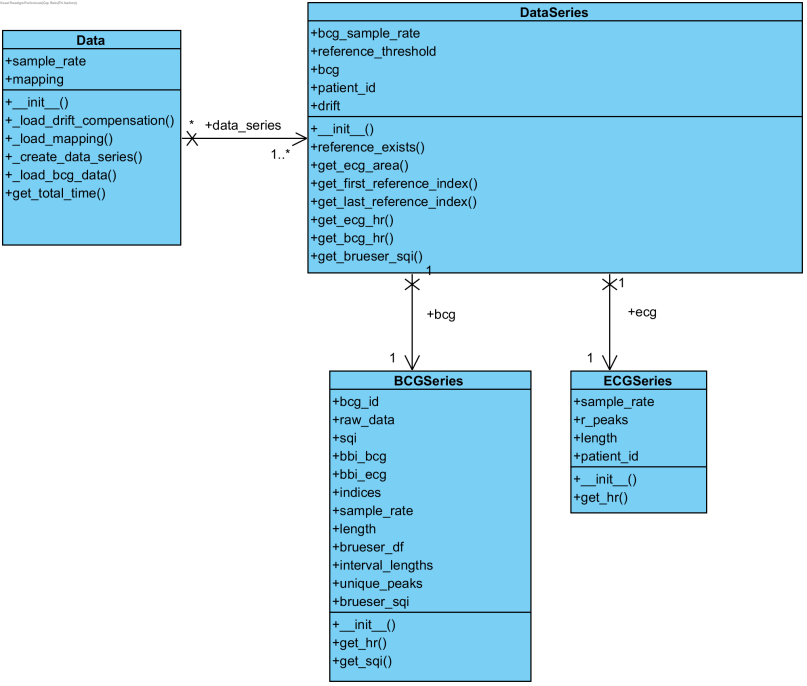
\includegraphics[width=0.9\textwidth]{pic/data-prep-class.png}
		\caption[Klassendiagramm der Datenstruktur für die Messdaten]{Klassendiagramm der Datenstruktur für die Messdaten}
		\label{fig:data-prep-class}
	\end{figure}
	
	Um die Herzraten auf Intervallen bestimmen zu können, müssen sowohl das \ac{BKG}- als auch das \ac{EKG}-Signal vorverarbeitet werden. Da diese Vorverarbeitung durch die große Datenmenge sehr aufwändig ist, werden die Ergebnisse als .csv-Dateien serialisiert. Beim Laden der Prüfen kann so geprüft werden, ob die Berechnung wiederholt werden muss oder geladen werden kann.
	
	Bei der Vorverarbeitung des \ac{BKG}-Signals wird der in Kapitel \ref{CLIE} vorgestellte CLIE-Algorithmus angewendet und die ermittelten Indices der Intervalle, die geschätzte Intervallängen und der in Kapitel \ref{brueserQI} beschriebene Qualitätsindex gespeichert. Für das \ac{EKG}-Signal wird für die alle drei Kanäle eine Detektion der QRS-Komplexe durchgeführt, mit denen die Schlag-zu-Schlag Intervalle ermittelt werden können. Dafür wird die Python-Implementierung von \citeauthor{Howell2019} des von \citeauthor{Elgendi2010} beschriebenen Algorithmus\footcite[][]{Elgendi2010} genutzt. Dieser zeigt in einer Untersuchung von \citeauthor{Porr2019} gute Ergebnisse.\footcite[Vgl.][]{Porr2019}
	
	
	\subsection{Annotation der Daten}
	
	Die vorliegenden Daten sind nicht annotiert. Es ist im Rahmen dieser Arbeit nicht möglich, die Annotation durch Expert*innen durchführen zu lassen, weshalb auf das parallel aufgenommene \ac{EKG} zurückgegriffen wird. Aufgrund des nicht-linearen Drifts der Daten ist eine herzschlaggenaue Synchronisierung schwierig. Aus diesem Grund wurde entschieden, die Annotation bereichsweise vorzunehmen. Für jeden Bereich wird zunächst geprüft, ob aussagekräftiges Referenzsignal existiert. Falls nicht, wird der entsprechende Bereich ausgeschlossen und nicht weiter verwendet. Ansonsten wird die durchschnittliche Herzrate sowohl für BKG- als auch EKG-Signal berechnet. Für die Berechnung der Herzfrequenz im \ac{BKG} wird der Median der geschätzten Intervalllängen verwendet. So werden Ausreißer weniger stark gewichtet.
	
	Auch bei dem Referenzsignal wird die Herzrate über den Median der Intervalllängen ermittelt. Die Intervalllängen entsprechen hier den Abständen der ermittelten R-Peaks. Da drei \ac{EKG}-Kanäle vorliegen, wird die Herzrate zunächst für jeden Kanal einzeln geschätzt. Falls die geschätzte Herzrate außerhalb des erwarteten Bereichs von 30 bis 200 Schlägen pro Minute liegt, wird der Kanal verworfen. Die Auswahl des Kanals gestaltet sich schwieriger, da auch im Referenzsignal teilweise schlechtes Signal vorliegt. Um dies auszugleichen, wird zur Auswahl des Kanals die Herzrate ebenfalls auf einem doppelt so großem Fenster berechnet. Von diesen drei Herzraten wird die ausgewählt, deren Kanal die geringste Spannweite an Intervalllängen aufweist. Mit Hilfe der geschätzten Herzrate des größeren Fensters wird nun der Kanal für die endgültige Schätzung ausgewählt, der die geringste Abweichung zu der Schätzung des größeren Fensters hat. Die Auswirkungen dieses Verfahrens sind in Abbildung \ref{fig:ecg-patient-26} sichtbar. Eine Fusionierung nur auf dem aktuellen Bereich führt zu einigen Fehlern in der Herzratenschätzung, die die Umgebung einbeziehende Fusionierung führt zu deutlich besseren Ergebnissen. Auch ist hier sichtbar, wie groß die Abweichung einzelner Kanäle ist.
	
	\begin{figure}[H]
		\centering
		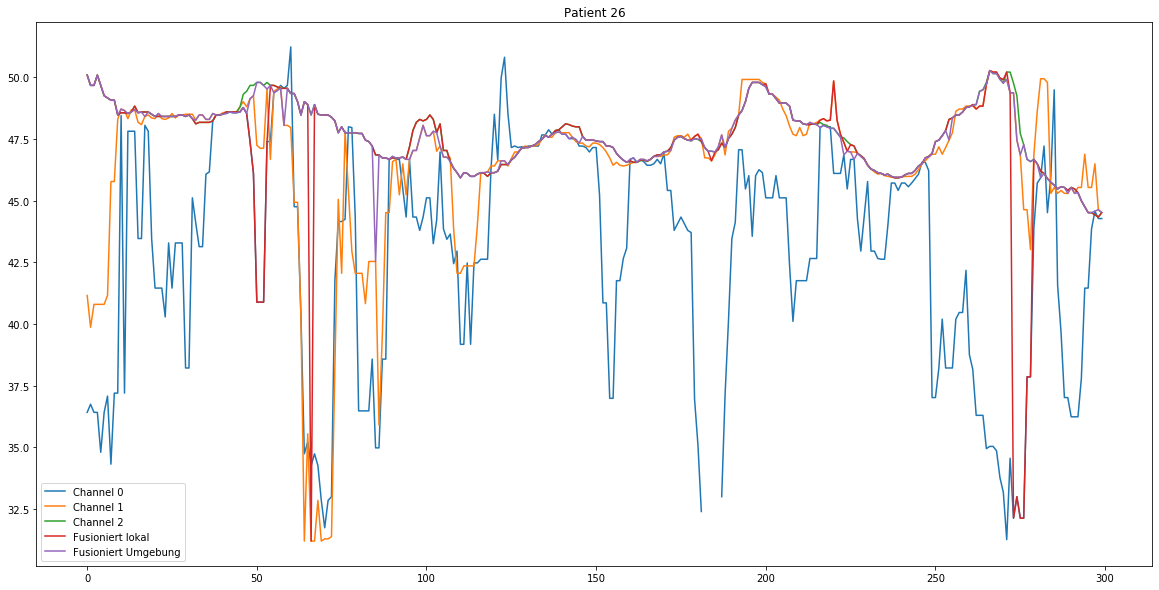
\includegraphics[width=0.95\textwidth]{pic/ecg-patient-26.png}
		\caption[\ac{EKG}-Herzratenschätzungen auf sich überlappenden 10-Sekunden-Segmenten für Patient 26]{\ac{EKG}-Herzratenschätzungen auf sich überlappenden 10-Sekunden-Segmenten für Patient 26. Fusioniert lokal zeigt die Fusionierung ohne Miteinbeziehung der Umgebung, Fusioniert Umgebung die oben beschriebene Fusionierung}
		\label{fig:ecg-patient-26}
	\end{figure}


	% TODO: Referenz Norm
	Auf Basis dieser beiden Herzraten wird nun die Annotation vorgenommen. Dabei wurde sich an der Norm für \ac{EKG}-Patientenmonitoren orientiert. Diese schreibt vor, dass die Abweichung der Herzrate maximal 10 \% oder 5 Schläge pro Minute betragen darf, je nachdem welcher der beiden Werte größer ist\footcite[]{} und wurde hier so übernommen. Wenn eine höhere oder niedrigere Genauigkeit gefordert ist, kann dies auch auf 15 \% und 7.5 Schläge pro Minute oder 5 \% und 2.5 Schläge pro Minute angepasst werden. Die entsprechenden Verteilungen der Labels für 10 Sekunden lange Segmente mit 90 \% Überlappung für 5, 10 und 15 \% maximale Abweichung sind in Abbildung \ref{fig:label-distribution} zu sehen.
	
	\begin{figure}[H]
		\centering
		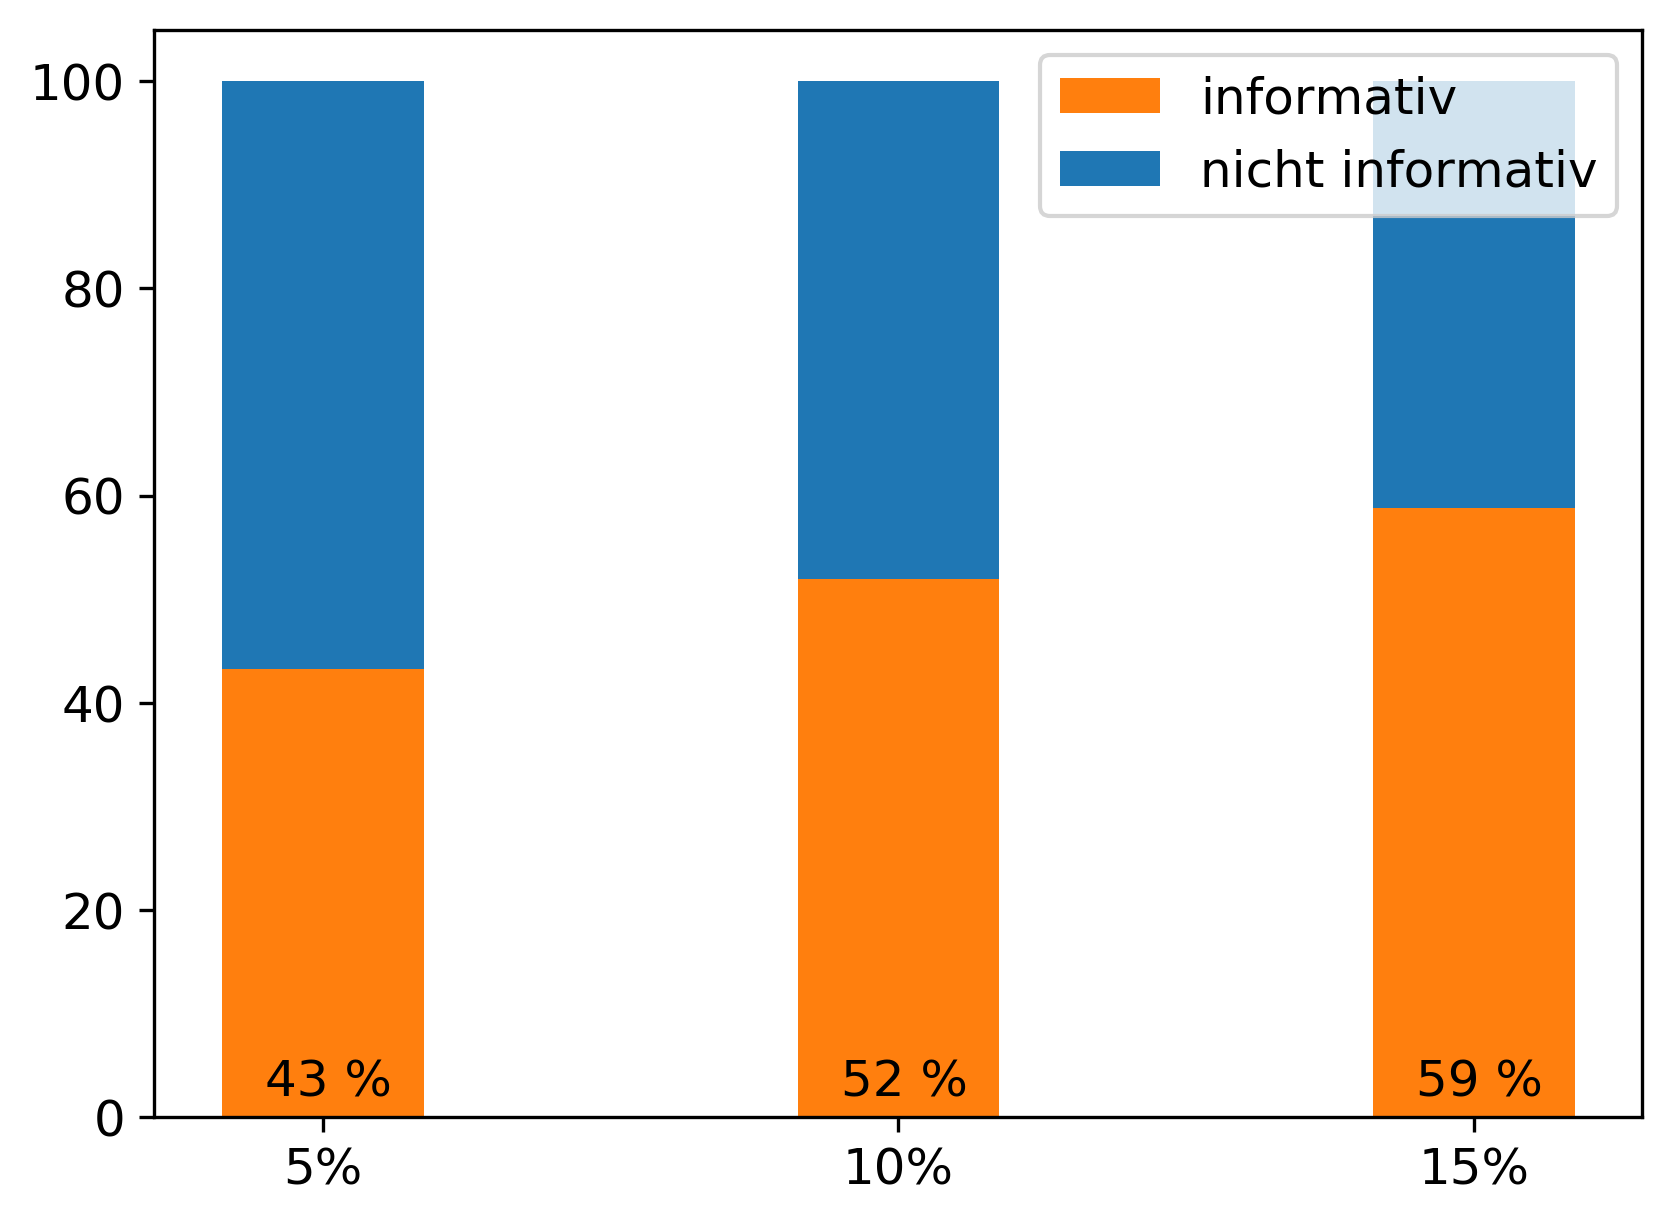
\includegraphics[width=0.55\textwidth]{pic/label-distribution.png}
		\caption[Verteilung der Label je nach maximal zulässiger Abweichung]{Verteilung der Label je nach maximal zulässiger Abweichung}
		\label{fig:label-distribution}
	\end{figure}
	
	Es ist auffällig, dass die Anteile des informativen Segments stark patient*innenabhängig sind. In Abbildung \ref{fig:data-stats-15} wird dies für 10 \% maximale Abweichung visualisiert.
	
	
	\begin{figure}[H]
		\centering
		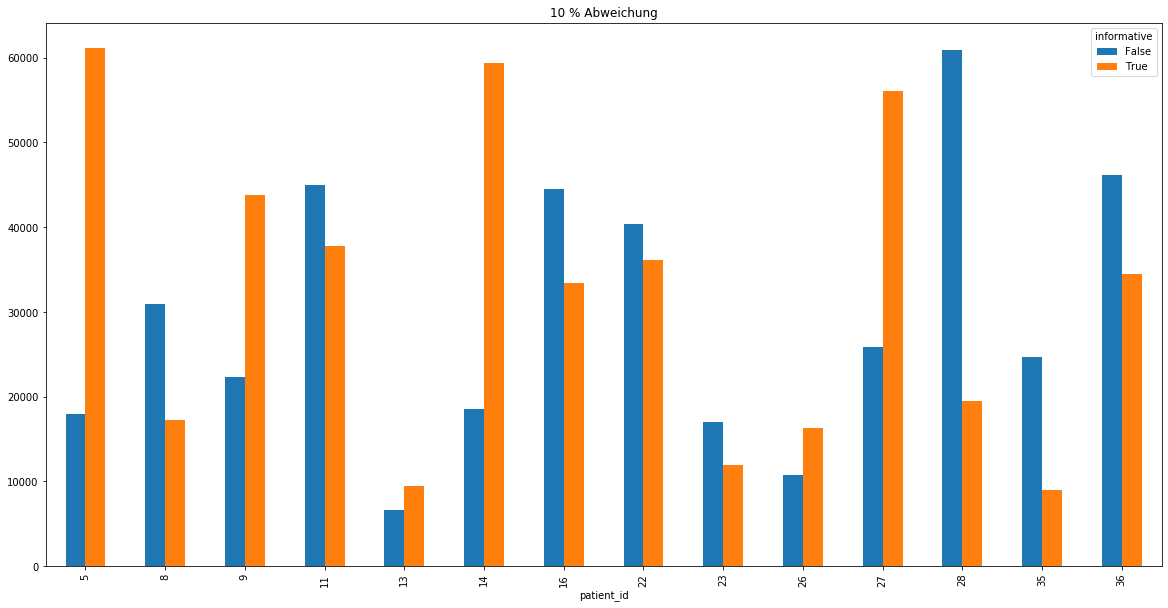
\includegraphics[width=0.9\textwidth]{pic/data-stats-10.png}
		\caption[Verteilung der Label pro Patient*in]{Verteilung der Label pro Patient*in}
		\label{fig:data-stats-15}
	\end{figure}
		

